\section{Evaluation} \label{sec:Evaluation}

In dem vorliegenden Kapitel wird kurz die Durchführung der Versuchsreihe beschrieben und die Evaluierung der Ergebnisse des Versuchssystems durchgeführt.
Hierzu werden die Ergebnisse aufbereitet und anhand mehrerer Metriken verglichen.

Das Versuchssystem wird über das Ausführen der \codestyle{main.py}-Datei gestartet (siehe linke Lane im Sequenzdiagramm (Abbildung \ref{fig:sequenzdiagramm-versuchssystem})).
Hier lässt sich spezifizieren, welche der Konfigurationen bei der aktuellen Ausführung analysiert werden sollen, wie man in Zeile~\ref{line:runrange} des Listing~\ref{lst-mainpy} erkennen kann.

\begin{lstlisting}[language=Python,caption=Ausführen einer Versuchsreihe,label=lst-mainpy,escapechar=|]
# load configs from json file
configs = []
with open(os.path.join(os.path.dirname(__file__), "Configs", "configs.json"), "r") as json_file:
    configs = json.load(json_file)

# range for current run
controller = Controller(os.path.join(os.path.dirname(__file__), "results.csv"))
for i in range(0, 20): |\label{line:runrange}|# range for current run
    controller.set_config(configs[i])
    controller.start()
\end{lstlisting}

Da die Analyse von einer Konfiguration im Durchschnitt etwa 35 Minuten dauert, werden die Konfigurationen auf mehrere Geräte aufgeteilt. 
Es kommen insgesamt fünf verschiedene Geräte mit unterschiedlicher Leistung zum Einsatz, die die Konfigurationen blockweise abarbeiten.
Der gesamte Prozess dauert ca. eineinhalb Wochen, wobei zu beachten ist, dass die verwendeten Geräte nicht rund um die Uhr rechnen.
Die Ergebnisse der Analysen werden in CSV-Dateien geschrieben, welche nach dem Beenden der Berechnungen zusammengeführt werden.

\textauthor{\vJB}{}{}

Für die Auswertung der Zuordnungsverteilungen aller Konfigurationen des Versuchssystems werden die Ergebnisse zunächst grafisch dargestellt.
Dabei werden in allen Grafiken die Ergebnisse der drei neuronalen Netze pro Konfiguration miteinander verrechnet.
Es werden vier verschiedene Aspekte betrachtet (vgl. Abbildung~\ref{fig:AuswertungVersuchssystem}).
\begin{figure}[H]
    \centering
    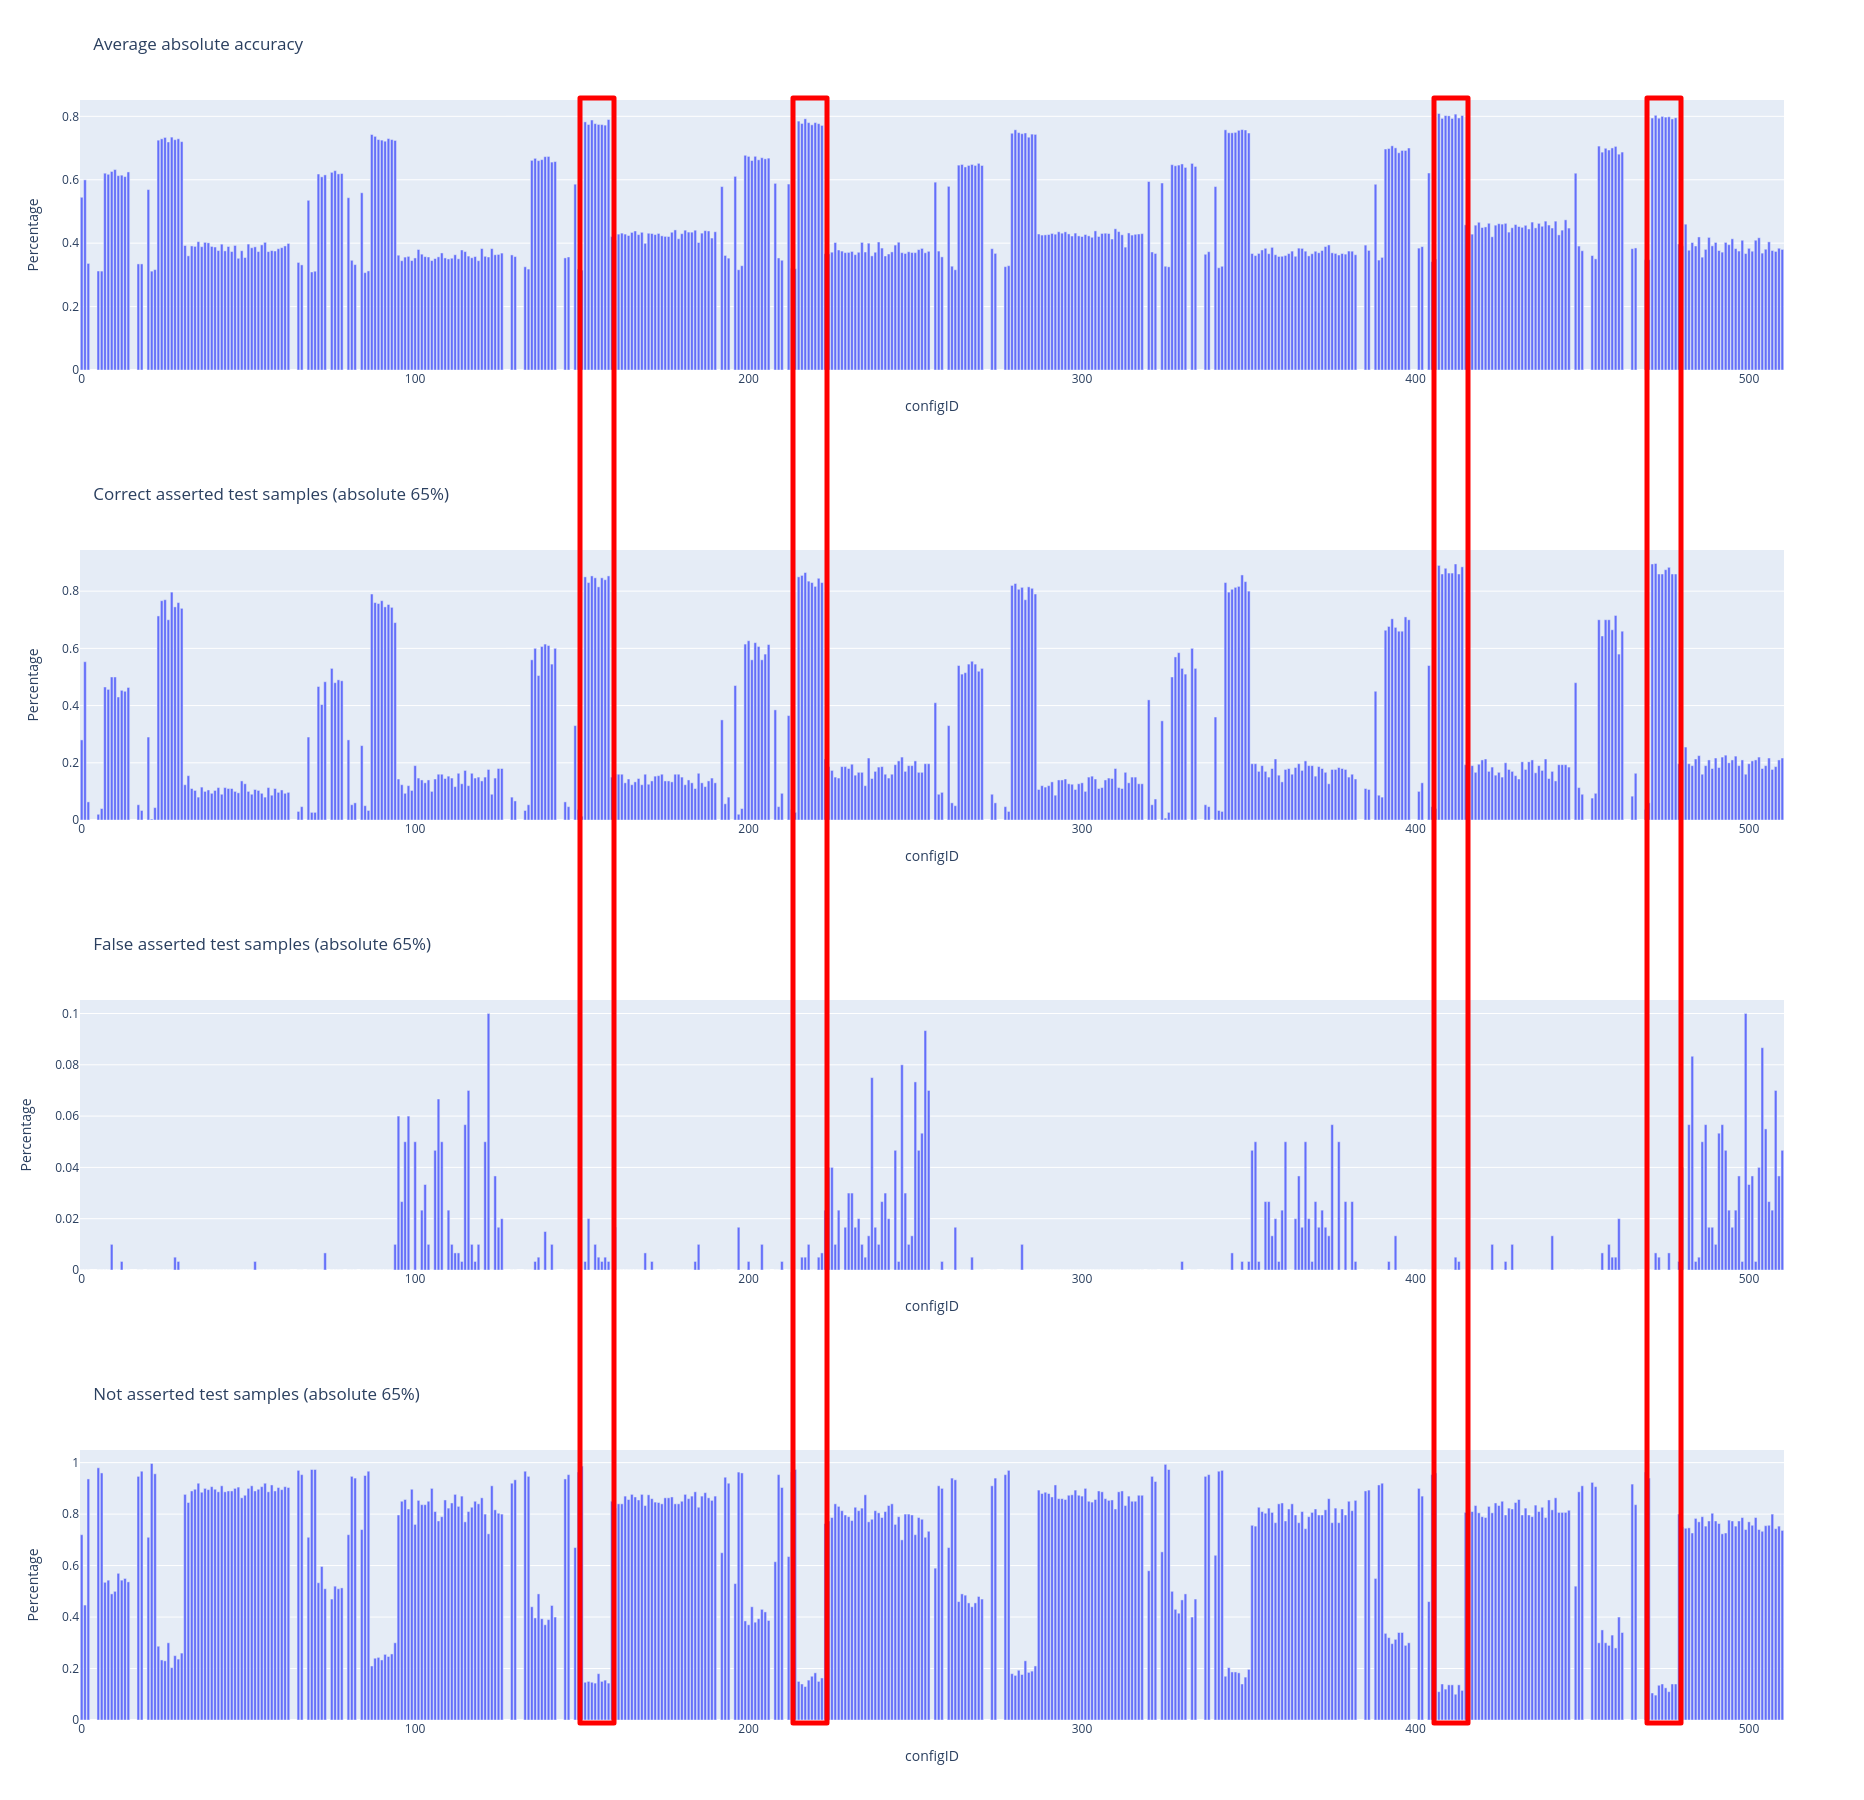
\includegraphics[width=1\textwidth, keepaspectratio]{images/Auswertung.png}
    \caption{Auswertung Versuchssystem}
    \label{fig:AuswertungVersuchssystem}
\end{figure}

Für die durchschnittliche absolute Genauigkeit (erstes Diagramm) werden die Wahrscheinlichkeiten für den zu identifizierenden Benutzer pro Testdatei aufsummiert und der Durchschnitt gebildet.
Eine Genauigkeit von 80 \% entspricht damit der Aussage, dass das neuronale Netz in Kombination mit der jeweiligen Konfiguration dem zu authentifizierenden Benutzer im Durchschnitt 80 \% der Frames der Testdatei zuordnet.

% TODO: Eingehen auf Closed-Set sobald die Entscheidung im Konzept beschrieben ist (Threshold)
Bereits in dieser Grafik zeigt sich die Bildung von Clustern.
Die besten Konfigurationen erreichen eine Genauigkeit von über 65 \%, weshalb dieser Wert für die folgenden drei Auswertungen verwendet wird.
Hier werden die Testdateien mittels dieses Wertes in die drei Kategorien korrekt zugeteilt, falsch zugeteilt und nicht zugeteilt eingeordnet.

Eine Testdatei gilt als korrekt zugeteilt, wenn dem zu authentifizierenden Benutzer mindestens 65 \% der Frames zugeordnet werden.
Analog gilt die Testdatei als nicht korrekt zugeteilt, wenn einem anderen Benutzer mindestens 65 \% der Frames zugeordnet werden.
Erreicht kein Nutzer mindestens 65 \%, so wird die Testdatei als nicht zugeteilt eingestuft.

Für die Bewertung der Konfigurationen gibt es grundsätzlich zwei unterschiedliche Ansätze.
Zunächst kann eine Konfiguration anhand der Anzahl an richtig zugewiesenen Samples bewertet werden.
Dabei steht der Fokus besonders darauf, dass möglichst viele Sprecher möglichst zuversichtlich erkannt und damit auch authentifiziert werden.
In dieser Betrachtung wird allerdings die Anzahl an falsch, beziehungsweise nicht zugewiesenen Samples vernachlässigt, was bedeutet, dass es trotz einer hohen Anzahl an richtigen Zuweisungen auch eine verhältnismäßig hohe Anzahl an falschen Zuweisungen geben kann.
Dies bedeutet für das System, dass die Wahrscheinlichkeit erhöht ist, dass sich eine Person als einen anderen Benutzer ausgeben und authentifizieren kann.

Der dazu gegenteilige Ansatz fokussiert sich auf die Anzahl der falsch zugeordneten Samples.
Um das System möglichst sicher zu halten, sollte diese Zahl minimal (im Optimalfall null) sein.
Es wird also sichergestellt, dass sich keine Person als ein anderer Benutzer erfolgreich authentifizieren kann.
Im Gegenzug kann dies jedoch bedeuten, dass die Anzahl an richtig zugewiesenen Samples sinkt, beziehungsweise die Anzahl der nicht zugewiesenen Samples steigt.
Somit ist die Wahrscheinlichkeit erhöht, dass ein Authentifizierungsversuch trotz korrektem Sprecher fehlschlägt und gegebenenfalls öfters wiederholt werden muss.

Für die Bewertung der Ergebnisse zum Einsatz in dem in dieser Arbeit entwickelten Demosystem wird eine Kombination der beiden Ansätze verfolgt.
Priorisiert wird hierbei der erste Ansatz, also die Orientierung an dem Datensatz mit den Meisten richtig zugeordneten Testdateien um eine gute Benutzerfreundlichkeit zu erzielen.
Gleichzeitig wird aber auch darauf geachtet, dass die Anzahl der falsch zugeordneten Samples möglichst gering ist.
Der Anzahl der nicht zugewiesenen Samples wird eine geringe Wichtigkeit zugeschrieben, da durch die Optimierung der zwei anderen Werte automatisch ein akzeptabler Wert gewährleistet ist.
Außerdem sind die Folgen einer hohen Anzahl nicht zugeordneter Sample vergleichsweise gering, da zunächst keine Authentifikation stattfindet und die Authentifikation mit einem neuen Testsample wiederholt werden kann.

Unter Betrachtung der durchschnittlichen absoluten Genauigkeit, sowie der korrekt zugeteilten Testdateien (zweites Diagramm), ergeben sich die vier markierten Cluster als beste Konfigurationen.
Auch in den zwei verbleibenden Kategorien, zeichnen sich diese Konfigurationen vor allem durch eine niedrige Anzahl an nicht zugeordneten Dateien (kleiner 25 \%, viertes Diagramm), sowie falsch zugeordneter Dateien (kleiner 2 \%, drittes Diagramm) aus.

Die Bildung der Cluster ist dabei auf die Art und Weise wie die Konfigurationen erzeugt werden zurückzuführen.
Da hier eine bestimmte Systematik vorliegt, enthalten diese Cluster jeweils ähnliche Feature-Kombinationen, wobei die für die Ergebnisse relevanten Features in jeder Konfiguration des Clusters vorhanden sind.
In den rot markierten Clustern sind dies \ac{MFCC} und \ac{dMFCC} Features.

In einer detaillierteren Analyse im Direktvergleich ergeben sich die in Tabelle~\ref{table:ergebnisOutput} dargestellten Konfigurationen als beste Kombinationen:
\begin{table}[H]
    \centering
    \begin{tabular}{c|c|c|c|c|c}
    ID  & Durchschnittliche absolute Genauigkeit & \ac{LPC} & \ac{MFCC} & \ac{LPCC} & \ac{dMFCC} \\ \hline
    472 &                                 0.8033 &        0 &        20 &         0 &         13 \\ \hline
    474 &                                 0.8015 &        0 &        20 &        13 &         13 \\ \hline
    410 &                                 0.8015 &        0 &        20 &        13 &         13 \\ \hline
    408 &                                 0.7989 &        0 &        20 &         0 &         13 \\ \hline
    414 &                                 0.7986 &        0 &        20 &        13 &         13 \\
    \end{tabular}
    \caption{Auswertung der Konfigurationen}
    \label{table:ergebnisOutput}
\end{table}

Die Evaluation ergibt somit, dass die Konfiguration mit der ID 472 die besten Ergebnisse erzielt.
Dabei werden 15000 Frames bei einer Frame-Größe von 600 Samples generiert.
Daraufhin werden 20 \ac{MFCC} Koeffizienten, sowie 13 \ac{dMFCC} Koeffizienten pro Frame erzeugt, welche durch das neuronale Netz ausgewertet werden.
\ac{LPC} und \ac{LPCC} zeigen in den ausgewählten Konfigurationen keinen signifikanten Mehrwert, weshalb diese nicht verwendet werden.

In einem weiteren Schritt werden basierend auf der Konfiguration 472 weitere Konfigurationen erstellt, um zusätzliche Untersuchungen durchzuführen.
Dabei werden die Parameter Anzahl der Frames, Länge der Frames, sowie Anzahl der \ac{MFCC} Koeffizienten um jeweils einen neuen Wert erweitert, da hier zu erkennen ist, dass eine Erhöhung dieser Werte zu einer Verbesserung des Gesamtergebnisses führt.
Folgend werden die Parameterwerte 20000 Frames, 800 Samples pro Frame und 27 \ac{MFCC} Koeffizienten evaluiert.
Die Parameterverteilung der Konfigurationen sind in Tabelle~\ref{table:additionalKonfigs} dargestellt.
\begin{table}[H]
    \centering
    \begin{tabular}{c|c|c|c|c}
    ID  & Anzahl Frames & Länge Frames & \ac{MFCC} & \ac{dMFCC} \\ \hline
    511 & 20000         & 600          & 20        & 13         \\ \hline
    512 & 15000         & 800          & 20        & 13         \\ \hline
    513 & 15000         & 600          & 27        & 13         \\ \hline
    514 & 20000         & 800          & 20        & 13         \\ \hline
    515 & 20000         & 600          & 27        & 13         \\ \hline
    516 & 15000         & 800          & 27        & 13    
    \end{tabular}
    \caption{Zusätzliche Konfigurationen}
    \label{table:additionalKonfigs}
\end{table}
Die Ergebnisse der Konfigurationen sind in Tabelle~\ref{table:resultAdditionalKonfigs} aufgelistet.
Da wie bereits beschrieben die Anzahl an richtig zugeordneten Samples in der Evaluierung bevorzugt wird, ergibt sich ein neues optimales Modell mit der Konfigurations-ID 516.
Dabei kann ein Anstieg der richtig zugeordneten Samples um 2,6 Prozentpunkte verzeichnet werden.
Diese Verbesserung ist damit auf die Erhöhung der Framelänge, sowie der Anzahl an \ac{MFCC} Koeffizienten zurückzuführen.

\begin{table}[H]
    \centering
    \begin{tabular}{c|c|c|c|c}
        ID            & Durchschn. abs. Genauigkeit & Richtig zug.   & Falsch zug.    & Nicht zug.     \\ \hline
        472           & 0,8033                      & 0,897          & 0,007          & 0,097          \\ \hline \hline
        511           & 0,8123                      & 0,885          & 0,005          & 0,110          \\ \hline
        512           & 0,8159                      & 0,885          & 0,010          & 0,105          \\ \hline
        513           & 0,8083                      & 0,880          & \textbf{0,003} & 0,117          \\ \hline
        514           & \textbf{0,8416}             & 0,900          & 0,007          & 0,093          \\ \hline
        515           & 0,8190                      & 0,877          & 0,007          & 0,117          \\ \hline
        \textbf{516}  & 0,8377                      & \textbf{0,923} & 0,007          & \textbf{0,070} \\ \hline \hline
        Diff 516-472  & +0,0344                     & +0,026         & 0,000          & -0,027
    \end{tabular}
    \caption{Ergebnisse der zusätzlichen Konfigurationen}
    \label{table:resultAdditionalKonfigs}
\end{table}
Dabei muss jedoch mit beachtet werden, dass mit dieser kleinen Verbesserung auch ein zusätzlicher Aufwand kommt.
Auf der einen Seite wird eine längere Audioaufzeichnung zur Authentifizierung benötigt, da die Framelänge um 200 Samples erhöht wird.
Auf der anderen Seite steigt auch der Rechenaufwand, da anstelle von 20 \ac{MFCC} Koeffizienten nun 27 Koeffizienten berechnet werden müssen.

Unter Anbetracht des erhöhten Aufwands wird somit von einer weiterreichenden Analyse mit mehr als 27 Koeffizienten abgesehen.
Da die Veränderungen die zu dem verbesserten Ergebnis führen für die einmalige Berechnung des Neuronalen Netzes des Demosystems tragbar sind, wird die für das Demosystem zu verwendende Konfiguration auf die Konfiguration mit der ID \textbf{516} festgelegt.

Um die Genauigkeit der Konfiguration für den Einsatz im Demosystem noch einmal zu erhöhen, wird das neuronale Netz erneut Trainiert, wobei die Epochen von 250 auf 500 erhöht werden.
Die Ergebnisse sind in Tabelle~\ref{table:resultsDemoSystemNN} aufgeführt.
Unter Verwendung des selben Thresholds von 65~\% wird eine weitere Verbesserung um 2,7 Prozentpunkte im Bereich der richtig zugeordneten Samples erreicht.

\begin{table}[H]
    \centering
    \begin{tabular}{c|c|c|c}
        Threshold & Richtig zug. & Falsch zug. & Nicht zug. \\ \hline
        65 \%     & 0,95         & 0,01        & 0,04       \\ \hline
        70 \%     & 0,90         & 0,00        & 0,10       \\ 
    \end{tabular}
    \caption{Ergebnisse des neuronalen Netz des Demosystems}
    \label{table:resultsDemoSystemNN}
\end{table}

Da die Anzahl an falsch zugeordneten Samples mit einem Prozentpunkt bereits sehr gering ist, kann hier durch eine Erhöhung des Thresholds das System im Bezug auf den Aspekt der Sicherheit weiter optimiert werden.
Durch die Erhöhung von 65~\% auf 70~\% werden keine Samples mehr falsch zugeordnet, gleichzeitig verschlechtert sich jedoch auch die Anzahl an richtig zugeordneten Samples.

Die Verschlechterung lässt sich durch zwei Aspekte rechtfertigen.
Auf der einen Seite ist es für Benutzer durch die Optimierung nicht mehr möglich, sich als eine andere Person zu authentifizieren.
Auf der anderen Seite sorgt die erhöhte Anzahl nicht zugeordneter Samples lediglich dafür, dass in 10~\% der Fälle eine erneute Aufzeichnung der Stimme für die Authentifizierung von Nöten ist.
Dieser Aufwand ist in Relation zu der gewonnenen Sicherheit sehr gering.

\textauthor{\vHS}{}{}